 
\documentclass[runningheads]{llncs}
\usepackage[english]{babel}
\usepackage{comment}
\usepackage{booktabs}
\usepackage{float}
\usepackage{listings}
\usepackage[T1]{fontenc}
% T1 fonts will be used to generate the final print and online PDFs,
% so please use T1 fonts in your manuscript whenever possible.
% Other font encondings may result in incorrect characters.
%
\pagestyle{plain}
\usepackage{graphicx}
\usepackage{hyperref}
\hypersetup{
    colorlinks=true,
    linkcolor=blue,
    filecolor=magenta,      
    urlcolor=cyan,
    pdftitle={Overleaf Example},
    pdfpagemode=FullScreen,
    }
\usepackage{comment}
% Used for displaying a sample figure. If possible, figure files should
% be included in EPS format.
%
% If you use the hyperref package, please uncomment the following two lines
% to display URLs in blue roman font according to Springer's eBook style:
%\usepackage{color}
%\renewcommand\UrlFont{\color{blue}\rmfamily}
%\urlstyle{rm}
%
\begin{document}
%
\title{Design and implementation of a probabilistic bird classification system based on selected modality and meta-information about the distribution of birds in geographical space}
%
%\titlerunning{Abbreviated paper title}
% If the paper title is too long for the running head, you can set
% an abbreviated paper title here
%
\author{Julianna Godziszewska}
%
\authorrunning{F. Author et al.}
% First names are abbreviated in the running head.
% If there are more than two authors, 'et al.' is used.
%
\institute{Wrocław University of Science and Technology}\\

%
\maketitle              % typeset the header of the contribution
%
\keywords{Machine Learning  \and Data Science \and Biodiversity.}

\section*{Abstract}

The aim of this work was to develop and evaluate a system of recognizing bird species based on recordings of their singing, with a focus on geographical location and its impact on classification. The study shows whether including spatial metadata enhances species recognition accuracy. To achieve this, two classification models were developed. One model is based on deep neural networks, which is responsible for species classification using spectrogram representations of bird sounds. Another one uses kernel density estimation to perform classification based on species occurrence coordinates and to model their geographical distribution at the same time. These models were integrated into a multi-classifier system to take advantage of their complementary strengths.\\

\section*{System architecture}

The system combines both acoustic and spatial information to improve classification performance. It consists of two models:
\begin{itemize}
    \item Model A is designed to classify audio data. It is implemented as a deep neural network consisting of convolutional layers.
    \item Model B is responsible for classifying geographical coordinates. It consists of kernel density estimators built separately for each class. For each class, a probability density function is estimated based on the training data. When a new sample is evaluated, each estimator calculates its density. The sample is then assigned to the class with the highest estimated density.
\end{itemize}
These two models are combined using an ensemble architecture. The final decision is made by a weighted average ensemble rule, where each expert, that is Model A and Model B contributes with a different weight.

\begin{figure}
    \centering
    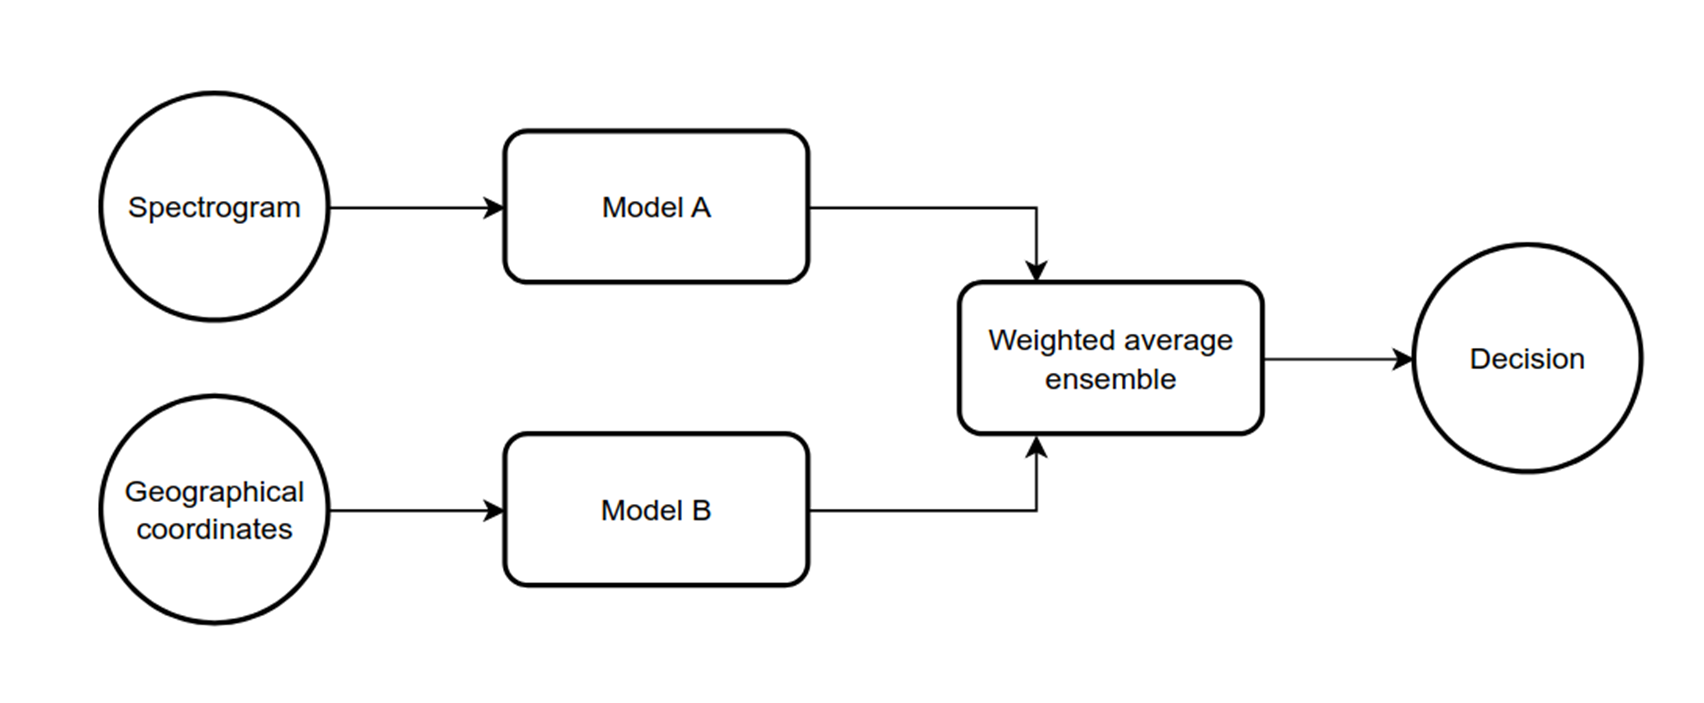
\includegraphics[width=1\linewidth]{images/image.png}
    \caption{System architecture}
\end{figure}

\section*{Data acquisition}
All the data that was used to build the bird recognition system comes from the Global Biodiversity Information Facility\footnotemar, which is an international and opensource network funded by the world's governments. It provides access to data about all types of life on Earth.
Downloaded data comes from six publicly available datasets and includes a total of 24 934 records:
\begin{itemize}
    \item Xeno-canto - Wildlife sounds from around the world \cite{Xeno-canto}
    \item iNaturalist Research - grade Observations \cite{inaturalist2024}
    \item Animal Sound Archive \cite{Animal_Sound_Archive}
    \item Observation.org, Nature data from around the World \cite{observation2024}
    \item My naturesounds - nature observations with sound recordings \cite{My_naturesounds}
    \item BoBO - Botanic Garden and Botanical Museum Berlin Observations \cite{botanicgarden2019}
\end{itemize}
All collected data consists of audio recordings, geographical coordinates and the bird species name. The dataset was filtered to include only bird species found in Poland, based on the geographical coordinates of the recordings.

\footnotetext{\url{https://gbif.com}}

\section*{Dataset}
In order to create the dataset for the system, the raw audio recordings  were converted into spectrograms, which represent a signal both in time and frequency domains.
The audio signal was sampled at a native sampling rate and then divided into time frames of size 2048 samples, with a hop size of 1024 samples. Each frame was smoothed using a Hanning window function to reduce spectral leakage during the frequency analysis. A Fast Fourier Transform was applied to convert each frame into the frequency domain. The resulting frequency representation was squared to obtain the power spectral density, which was then converted into a logarithmic scale to form the spectrogram\footnotemark. 

\footnotetext{\href{https://mlhive.com/2023/08/create-audio-spectogram-using-python}{Spectrogram code reference}}

\begin{figure}[H]
    \centering
    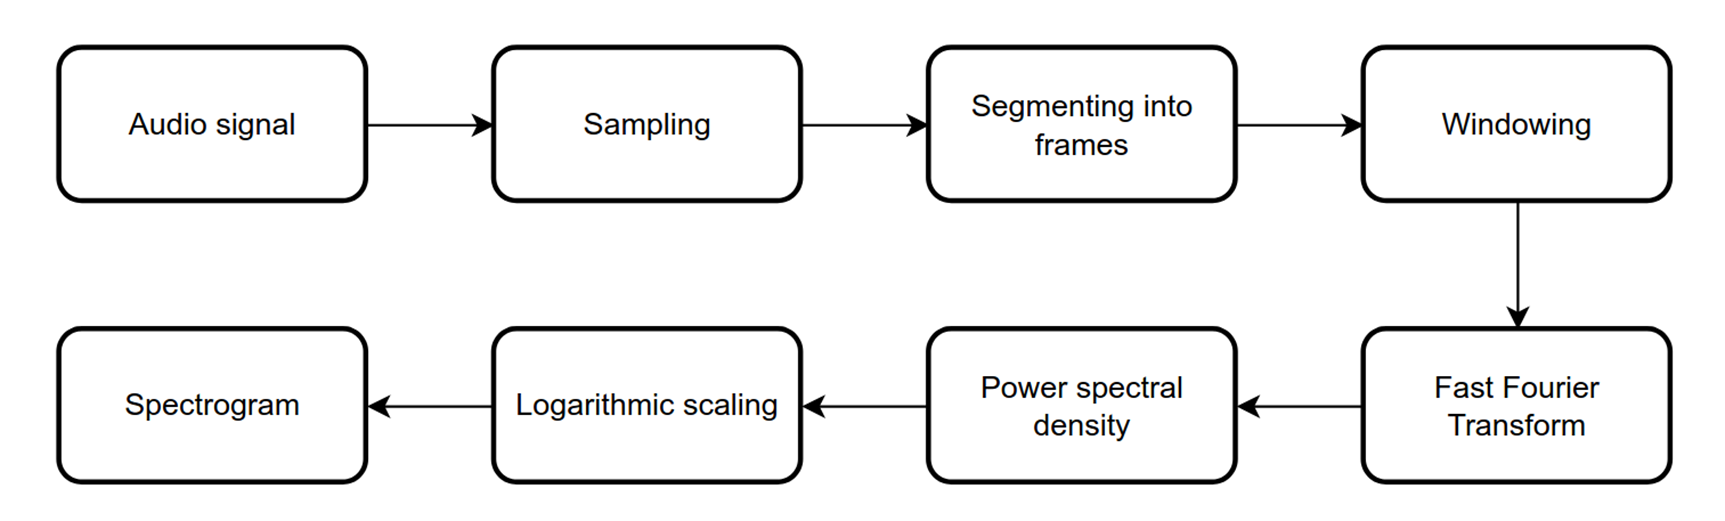
\includegraphics[width=1\linewidth]{images/image2.png}
    \caption{Process of generating a spectrogram}
\end{figure}

Due to the long duration of some recordings, it was necessary to divide the spectrograms into smaller segments in order to reduce the number of attributes. I decided to split the spectrograms every five frames and then flatten each segment into a one-dimensional vector. Each such spectrogram fragment is treated as a separate record, independent of other fragments from the same recording. \\

The dataset was split into three parts using stratified sampling to preserve the original class distribution across all subsets.
70\% of the data was used for training, 15\% for validation, and 15\% for testing.\\

The chart below (Fig. ~\ref{apriori}) presents the a priori class probability distribution, based on dataset occupancy for each class. The dataset consists of 306 classes, and as shown, the class distribution is heavily imbalanced. We can observe that a small number of classes dominate the dataset, while most classes have very low representation.
The classes are sorted in descending order based on their dataset occupancy, so the most frequent classes appear on the left side of the plot.

\begin{figure}[H]
    \centering
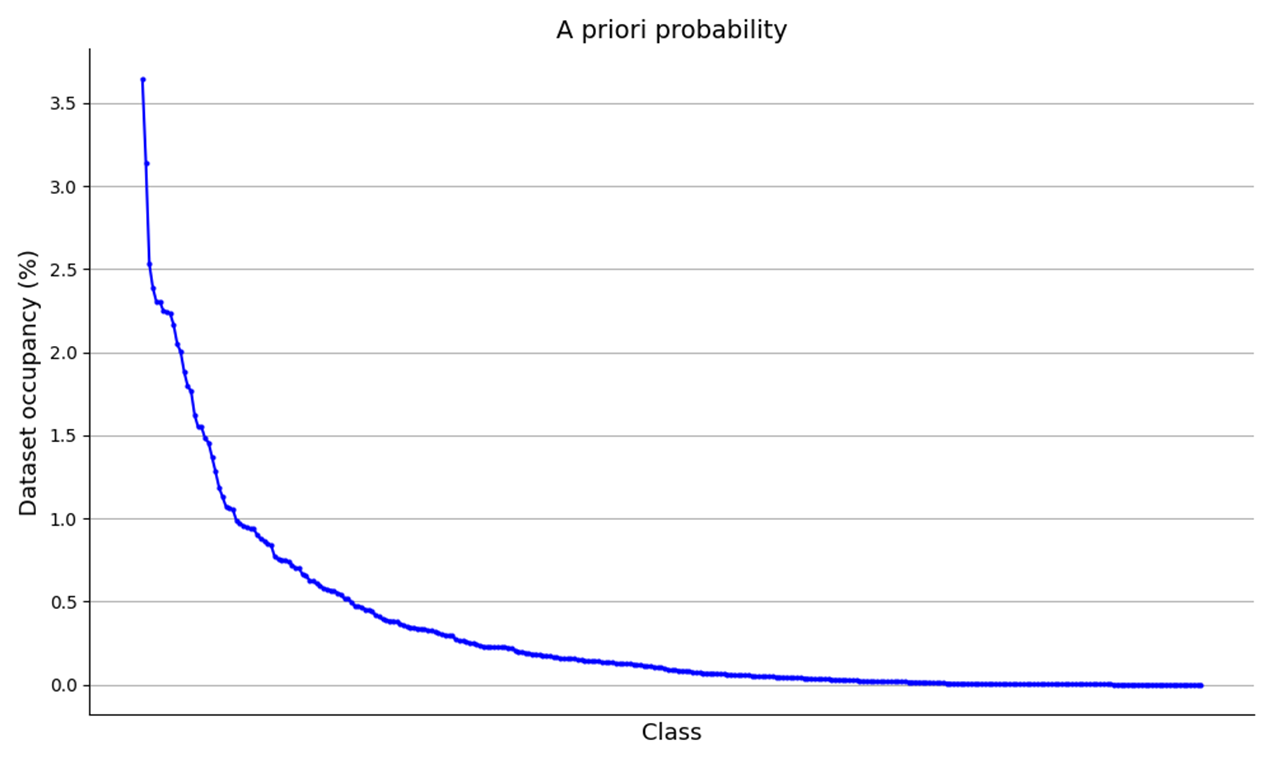
\includegraphics[width=1\linewidth]{images/image7.png}
    \caption{Dataset ocuppancy for each class}
    \label{apriori}
\end{figure}

\section*{Model A}

Model A focuses on the classification of audio recordings. It is built as a deep neural network that consists of four convolutional layers grouped with max-pooling operations, followed by fully connected layers\footnotemark.\\
The model uses ReLU as the activation function and applies log-softmax at the output to produce class probabilities.

\footnotetext{\href{https://pyimagesearch.com/2021/07/19/pytorch-training-your-first-convolutional-neural-network-cnn/}{CNN code reference}}


\noindent Due to the large size of the dataset, the training time was significant — each epoch took over 8 hours on average on available the equipment. Therefore, the model was trained for only 8 epochs.\\

\begin{figure}[H]
    \centering
    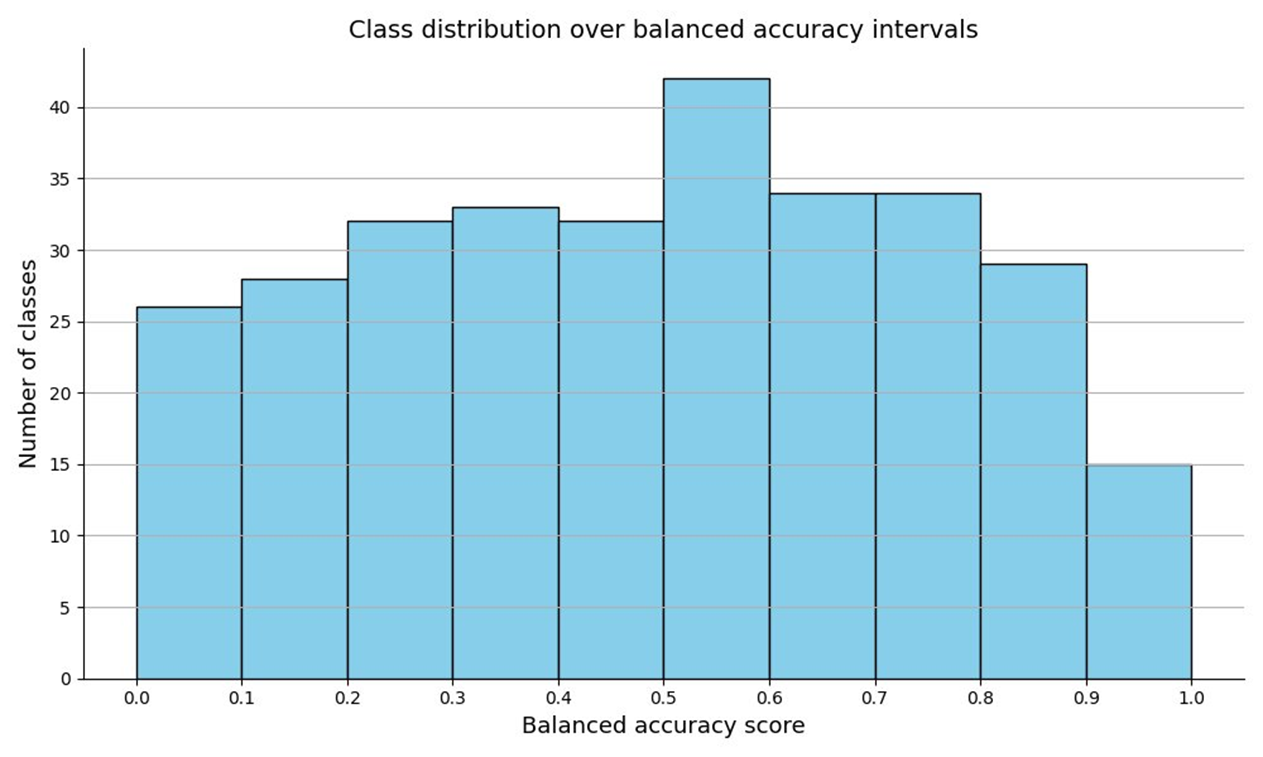
\includegraphics[width=1\linewidth]{images/image5.png}
    \caption{Class distribution over balanced accuracy scores of model A}
    \label{hist1}
\end{figure}

\noindent The histogram above (Fig. ~\ref{hist1}) shows the distribution of classes across intervals of the balanced accuracy score.
The distribution appears relatively even.
The least frequent result is in the 90\% to 100\% range, where only 15 classes reached this level of performance.

\section*{Model B}

Model B is designed to classify samples based on their geographical coordinates. It relies on kernel density estimation, where a separate density model is fitted for each class. The classification is performed by selecting the class with the highest estimated density for a given input location.

\begin{lstlisting}[language=Python, caption={Implementation of kernel density estimators}, captionpos=b]
from sklearn.neighbors import KernelDensity as KD

    def create_estimators(X_train, y_train, kernel):
    
        kde_estimators = {}
        unique_classes = np.unique(y_train)  
    
        for class_label in unique_classes:
            h = silverman_bandwidth(X_train[class_indices])
            kde = KD(kernel=kernel, bandwidth=h).fit(X_train[class_indices])  
            kde_estimators[class_label] = kde 
    
        return kde_estimators  
\end{lstlisting}
\bigskip
\begin{lstlisting}[language=Python, caption={Implementation of classification on test data}, captionpos=b]
import numpy as np

    def predict_classes(kde_estimators, X_test, y_test):

    predictions = []
    test_classes = np.unique(y_test)

    for sample in X_test:
        densities = {}

        for class_label, kde in kde_estimators.items():
            if class_label not in test_classes:
                continue  

            log_density = kde.score_samples(sample.reshape(1, -1))
            densities[class_label] = np.exp(log_density)  
            
        predicted_class = max(densities, key=densities.get)
        predictions.append(predicted_class)

    return np.array(predictions)
\end{lstlisting}



\noindent During the estimation of kernel density functions, it is very important to choose an appropriate kernel bandwidth parameter, which controls the level of smoothing applied to the distribution. I wanted to select a method that would best match my data.
Silverman's rule is a widely used method which is designed for unimodal, symmetric, and normally distributed data. \\
In my case, the input data consisted of raw geographical coordinates, which were not standardized or scaled.  Therefore, I decided to apply a modified version of Silverman’s rule, as it offers better robustness in the presence of outliers and can capture multimodal characteristics of the data more effectively.\\

\noindent That version of Silverman’s rule takes into account an additional measure of data dispersion — the interquartile range. This measure is more resistant to outliers than the standard deviation. Additionally, this method includes a reduced coefficient of 0.9 instead of 1.06, which improves the identification of multimodal features. The modified version of Silverman’s rule is described by the following formula \cite{bandwidth}:
$$h = 0.9\cdot min \left( \sigma, \frac{IQR}{1.35} \right) n^{-\frac{1}{5}}$$ 
where:\\
$h$ -  kernel bandwidth,\\
$\sigma$ - standard deviation of the sample,\\
$IQR$ - interquartile range, i.e., the difference between the third quartile and the first quartile,\\
$n$ - number of samples in the dataset.\\

\noindent To illustrate the impact of kernel selection and bandwidth adjustment, a series of experiments were conducted. The first set of experiments compared all available kernel types in Scikit-learn\cite{scikit-learn} library using the bandwidth parameter determined by modified Silverman’s method. 

\begin{comment}
However, it is crucial to note that excessively reducing the kernel bandwidth may lead to overfitting and insufficient smoothing of the density estimation. An overly small bandwidth can result in overly localized estimates, reducing generalization capability and leading to unstable classification performance.\\
\end{comment}

\begin{table}[H]

    \centering
        \caption{Balanced accuracy scores for the bandwidth parameter \( h \) determined using Silverman's method for different kernel types}
        \label{tab:KDE1}
        \begin{tabular}{lc}
        \toprule
        \textbf{Kernel Type}        & \multicolumn{1}{l}{\textbf{Balanced Accuracy Score}} \\
        
        \midrule
        Gaussian (Gauss)            & 0.713 \%                                        \\
        Tophat (Rectangular)        & 0.369 \%                                        \\
        Epanechnikov                & 1.385 \%                                        \\
        Exponential                 & 1.112 \%                                        \\
        Linear                      & 1.598 \%                                        \\
        Cosine                      & 1.471 \%  \\ 
        \bottomrule
        \end{tabular}
\end{table}

The table (Table ~\ref{tab:KDE1}) shows balanced accuracy scores for all kernel types. The best result achieved linear kernel, reaching approximately 1.6 \% of accuracy. We can observe that all scores for different kernels are relatively low. They are not satysfying, therefore I started exploring how they could be improved. I decided to experiment with reducing the bandwidth values by several orders of magnitude, but still using the modified Silverman's rule.\\
Therefore, the same kernel types were tested with a reduced kernel bandwidth, decreased by two orders of magnitude.

\begin{table}[H]
    \centering
        \caption{Balanced accuracy scores for the bandwidth parameter \( h \) determined using Silverman's method, decreased by two orders of magnitude for different kernel types}
        \label{KDE2}
        \begin{tabular}{lc}
        \toprule
        \textbf{Kernel Type}        & \multicolumn{1}{l}{\textbf{Balanced Accuracy Score}} \\
        
        \midrule
        Gaussian (Gauss)            & 14.076 \%                                        \\
        Tophat (Rectangular)        & 14.238 \%                                        \\
        Epanechnikov                & 15.547 \%                                        \\
        Exponential                 & 14.970 \%                                        \\
        Linear                      & 15.938 \%                                        \\
        Cosine                      & 15.603 \%  \\ 
        \bottomrule
        \end{tabular}
\end{table}

The results from the table above (Table ~\ref{KDE2}) shows balanced accuracy scores for all kernel types after decreasing kernel bandwidth by two orders of magnitude.\\
All kernel types achieved noticeably higher balanced accuracy scores compared to the previous configuration. Again, the linear kernel achieved the best result, this time reaching approximately 16\% balanced accuracy.


\section*{Model C}
Model C is a mixture of experts that combines the predictions of two individual models: Model A and Model B. The final prediction is obtained as a weighted average of the outputs from these experts, where the weights can be adjusted to control each expert’s influence.\\

\noindent The heatmap below (Fig. ~\ref{heatmap}) illustrates the performance of the mixture of experts in terms of balanced accuracy, depending on two key parameters: the kernel bandwidth used in Model B and the weight assigned to expert A. I assumed that Model A acts as the dominant expert, so I considered expert A weights of 0.6, 0.7, 0.8, 0.9, and 1.

\begin{figure}[H]
    \centering
    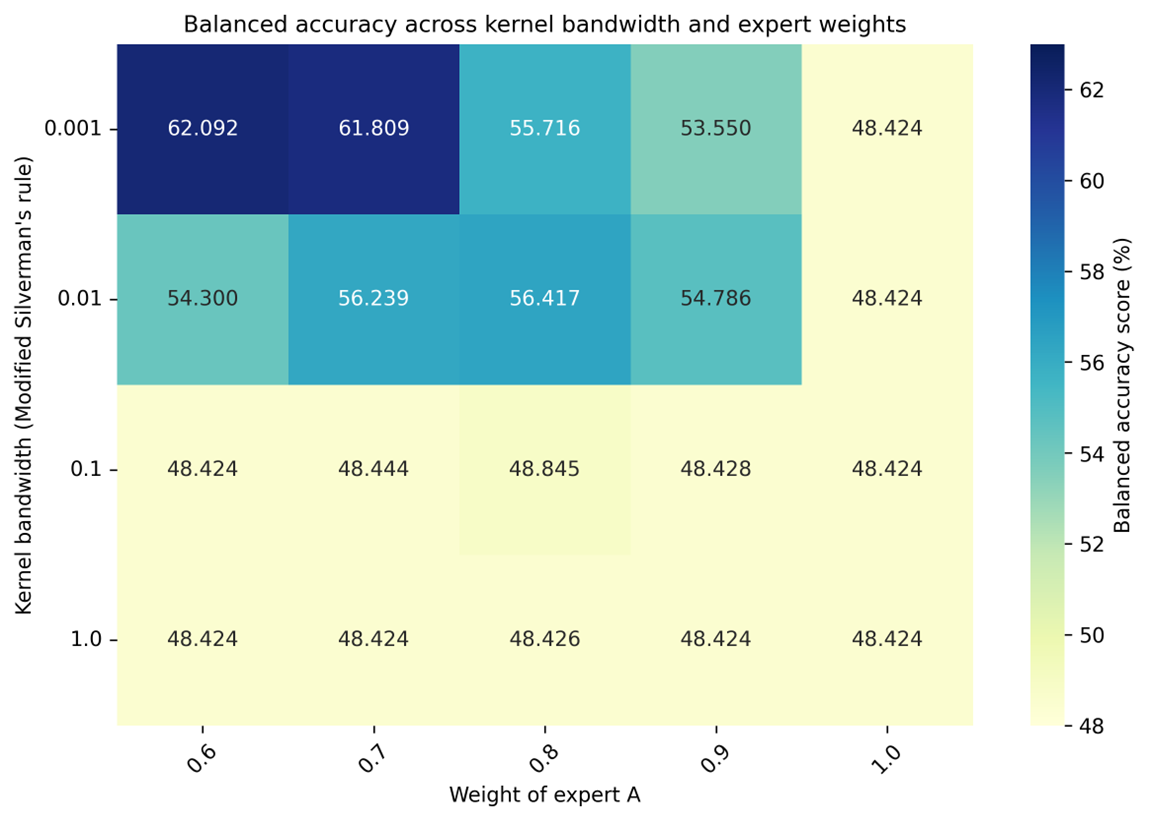
\includegraphics[width=1\linewidth]{images/image3.png}
    \caption{Impact of Kernel Bandwidth and Expert Weights on Balanced Accuracy}
    \label{heatmap}
\end{figure}

For the original modified Silverman's rule, as well as for the version scaled down by only one order of magnitude, the improvement in accuracy was minimal. 
The highest balanced accuracy score was achieved with a kernel bandwidth reduced by three orders of magnitude and an expert A weight of 0.6, reaching approximately 62.1\%.\\
However, despite this high score, I decided to reject this configuration due to the extremely low kernel bandwidth. I was concerned that the model might be overfitting to the training data. I decided to chose the smallest bandwidth value that enhanced the classification which is kernel bandwidth decreased by two orders of magnitude.
The final configuration of Model C used in the system was as follows:
\begin{itemize}
    \item Kernel bandwidth: modified Silverman’s rule, scaled down by two orders of magnitude,
    \item Kernel type: linear,
    \item Expert A weight: 0.8,
    \item Expert B weight: 0.2.
\end{itemize}	

The histogram below (Fig. ~\ref{hist2}) shows the distribution of the number of classes for each interval of the balanced accuracy score after applying Model C.
\begin{figure}[H]
    \centering
    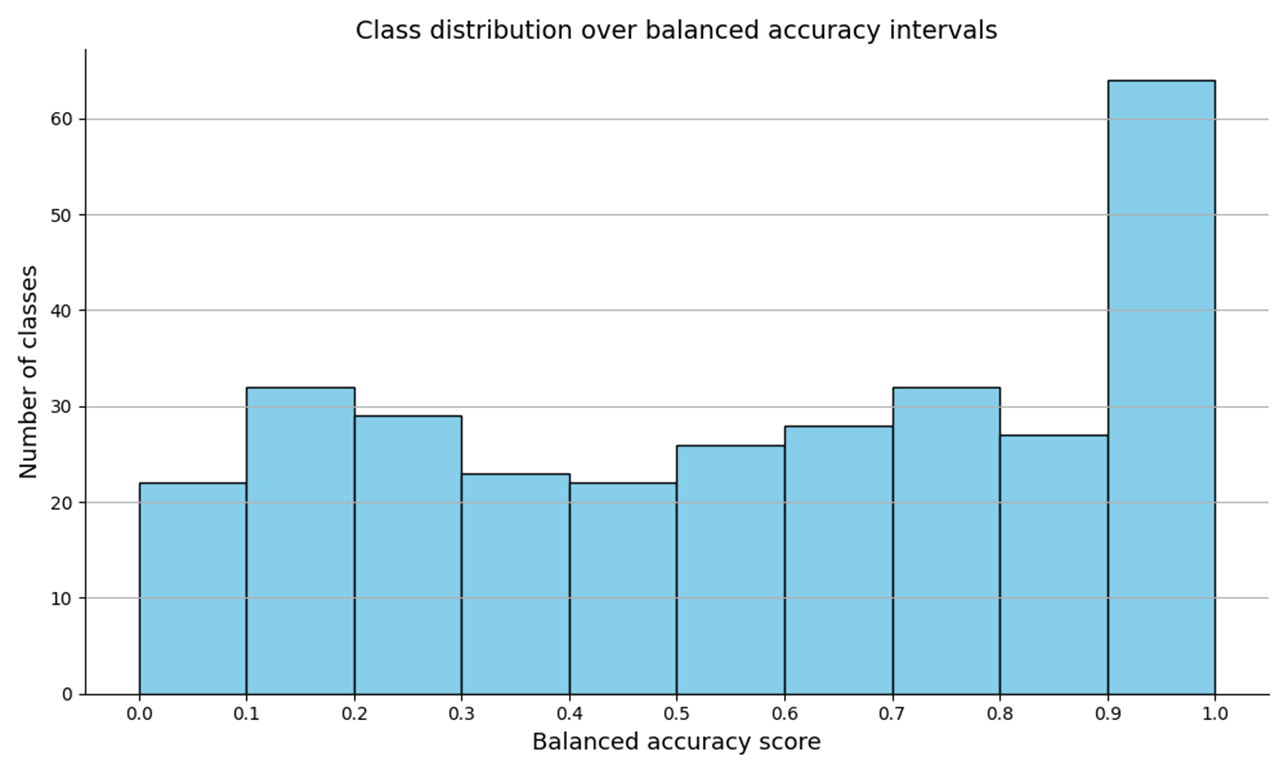
\includegraphics[width=1\linewidth]{images/image4.png}
    \caption{Class distribution over balanced accuracy scores intervals of model C}
    \label{hist2}
\end{figure}
Compared to the results for Model A, the number of classes that fall into the highest accuracy interval increased approximately four times.

\section*{Conclusions}

The main goal of this project was to develop a bird song recognition system using both audio recordings and geographical metadata. The system integrates two models into the mixture of experts that is able to classify spectrograms and location data. \\
\noindent Choosing the appropriate kernel bandwidth is crucial for obtaining a well-balanced density estimation. If parameter \textit{h} is too small, the model captures too many local variations, leading to overfitting and reduced generalization. On the other hand, an excessively large kernel bandwidth over-smooths the density function, making it difficult to distinguish between close data points. In practice, the kernel bandwidth can be interpreted as the "resolution" of the data: a smaller \textit{h} provides a high-resolution view with fine details, while a larger \textit{h} results in a low-resolution, more generalized representation of the distribution \cite{Combination_of__KDE_in_Classification}.\\
This effect was clearly observed in the performance of Model C. The results showed that reducing the kernel bandwidth parameter by two orders of magnitude led to a significant increase in classification performance, improving the balanced accuracy of the final system to approximately 56.4\%. Furthermore, the number of bird species recognized with near-perfect accuracy increased approximately four times compared to Model A alone.

\begin{comment}
\begin{table}
\caption{Table captions should be placed above the
tables.}\label{tab1}
\begin{tabular}{|l|l|l|}
\hline
Heading level &  Example & Font size and style\\
\hline
Title (centered) &  {\Large\bfseries Lecture Notes} & 14 point, bold\\
1st-level heading &  {\large\bfseries 1 Introduction} & 12 point, bold\\
2nd-level heading & {\bfseries 2.1 Printing Area} & 10 point, bold\\
3rd-level heading & {\bfseries Run-in Heading in Bold.} Text follows & 10 point, bold\\
4th-level heading & {\itshape Lowest Level Heading.} Text follows & 10 point, italic\\
\hline
\end{tabular}
\end{table}


\noindent Displayed equations are centered and set on a separate
line.
\begin{equation}
x + y = z
\end{equation}
Please try to avoid rasterized images for line-art diagrams and
schemas. Whenever possible, use vector graphics instead (see
Fig.~\ref{fig1}).

\begin{figure}

\includegraphics[width=\textwidth]{fig1.eps}
\caption{A figure caption is always placed below the illustration.
Please note that short captions are centered, while long ones are
justified by the macro package automatically.} \label{fig1}
\end{figure}

\begin{theorem}
This is a sample theorem. The run-in heading is set in bold, while
the following text appears in italics. Definitions, lemmas,
propositions, and corollaries are styled the same way.
\end{theorem}
%
% the environments 'definition', 'lemma', 'proposition', 'corollary',
% 'remark', and 'example' are defined in the LLNCS documentclass as well.
%
\begin{proof}
Proofs, examples, and remarks have the initial word in italics,
while the following text appears in normal font.
\end{proof}
For citations of references, we prefer the use of square brackets
and consecutive numbers. Citations using labels or the author/year
convention are also acceptable. The following bibliography provides
a sample reference list with entries for journal
articles~\cite{ref_article1}, an LNCS chapter~\cite{ref_lncs1}, a
book~\cite{ref_book1}, proceedings without editors~\cite{ref_proc1},
and a homepage~\cite{ref_url1}. Multiple citations are grouped
\cite{ref_article1,ref_lncs1,ref_book1},
\cite{ref_article1,ref_book1,ref_proc1,ref_url1}.

\begin{credits}
\subsubsection{\ackname} A bold run-in heading in small font size at the end of the paper is
used for general acknowledgments, for example: This study was funded
by X (grant number Y).

\subsubsection{\discintname}
It is now necessary to declare any competing interests or to specifically
state that the authors have no competing interests. Please place the
statement with a bold run-in heading in small font size beneath the
(optional) acknowledgments\footnote{If EquinOCS, our proceedings submission
system, is used, then the disclaimer can be provided directly in the system.},
for example: The authors have no competing interests to declare that are
relevant to the content of this article. Or: Author A has received research
grants from Company W. Author B has received a speaker honorarium from
Company X and owns stock in Company Y. Author C is a member of committee Z.
\end{credits}

%
% ---- Bibliography ----
%
% BibTeX users should specify bibliography style 'splncs04'.
% References will then be sorted and formatted in the correct style.
%
% \bibliographystyle{splncs04}
% \bibliography{mybibliography}
%
\begin{thebibliography}{8}
\bibitem{ref_article1}
Author, F.: Article title. Journal \textbf{2}(5), 99--110 (2016)

\bibitem{ref_lncs1}
Author, F., Author, S.: Title of a proceedings paper. In: Editor,
F., Editor, S. (eds.) CONFERENCE 2016, LNCS, vol. 9999, pp. 1--13.
Springer, Heidelberg (2016). \doi{10.10007/1234567890}

\bibitem{ref_book1}
Author, F., Author, S., Author, T.: Book title. 2nd edn. Publisher,
Location (1999)

\bibitem{ref_proc1}
Author, A.-B.: Contribution title. In: 9th International Proceedings
on Proceedings, pp. 1--2. Publisher, Location (2010)

\bibitem{ref_url1}
LNCS Homepage, \url{http://www.springer.com/lncs}, last accessed 2023/10/25
\end{thebibliography}
\end{comment}

%\pagestyle{bibliographyStyle}
\bibliographystyle{plainurl}
\bibliography{bibliography}
\end{document}
